\let\negmedspace\undefined
\let\negthickspace\undefined
\documentclass[journal]{IEEEtran}
\usepackage[a5paper, margin=10mm, onecolumn]{geometry}
%\usepackage{lmodern} % Ensure lmodern is loaded for pdflatex
\usepackage{tfrupee} % Include tfrupee package

\setlength{\headheight}{1cm} % Set the height of the header box
\setlength{\headsep}{0mm}  % Set the distance between the header box and the top of the text

\usepackage{gvv-book}
\usepackage{gvv}
\usepackage{cite}
\usepackage{amsmath,amssymb,amsfonts,amsthm}
\usepackage{algorithmic}
\usepackage{graphicx}
\usepackage{textcomp}
\usepackage{xcolor}
\usepackage{txfonts}
\usepackage{listings}
\usepackage{enumitem}
\usepackage{mathtools}
\usepackage{gensymb}
\usepackage{comment}
\usepackage[breaklinks=true]{hyperref}
\usepackage{tkz-euclide} 
\usepackage{listings}
% \usepackage{gvv}                                        
\def\inputGnumericTable{}                                 
\usepackage[latin1]{inputenc}                                
\usepackage{color}                                            
\usepackage{array}                                            
\usepackage{longtable}                                       
\usepackage{calc}                                             
\usepackage{multirow}                                         
\usepackage{hhline}                                           
\usepackage{ifthen}                                           
\usepackage{lscape}
\begin{document}

\bibliographystyle{IEEEtran}
\vspace{3cm}

\title{9.7.2.4}
\author{EE24BTECH11021 - Eshan Ray}

% \maketitle
% \newpage
% \bigskip
{\let\newpage\relax\maketitle}

\renewcommand{\thefigure}{\theenumi}
\renewcommand{\thetable}{\theenumi}
\setlength{\intextsep}{10pt} % Space between text and floats

\textbf{Question:}\\
For the Differential Equation $\brak{x^2 + y^2}\frac{dy}{dx} - xy=0$, verify that $x^2 = 2y^2\log{y}$ is a solution of the differential equation.

\solution{
Solving the given D.E. , we get,
\begin{align}
    \brak{x^2 + y^2}\frac{dy}{dx} - xy &=0 \\
    \implies    \frac{dy}{dx} &= \frac{xy}{x^2+y^2}\\
\end{align}
Substituting, $y = vx$, we get,
\begin{align}
    \implies    \frac{dy}{dx} &= v + x\frac{dv}{dx}\\
    \implies    v +x\frac{dv}{dx} &= \frac{x\brak{vx}}{x^2 + \brak{vx}^2}\\
    \implies    v + x\frac{dv}{dy} &= \frac{vx^2}{x^2\brak{1+v^2}}\\
    \implies    x\frac{dv}{dx} &= \frac{v}{1+v^2} -v\\
    \implies    x\frac{dv}{dx} &= \frac{v-v-v^3}{1+v^2}\\
    \implies    x\frac{dv}{dx} &= \frac{-v^3}{1+v^2}\\
    \implies    -\frac{\brak{1+v^2}dv}{v^3} &= \frac{dx}{x}\\
    \implies    -\frac{dv}{v^3} -\frac{v^2dv}{v^3} &= \frac{dx}{x}\\
\end{align}
Integrating both sides, we get,
\begin{align}
    \implies    -\int\frac{dv}{v^3}-\int\frac{dv}{v} &= \int\frac{dx}{x}\\
    \implies    \frac{1}{2v^2} - logv &= logx + C\\
\end{align}
putting $v = \frac{y}{x}$ we get,
\begin{align}
    \implies    \frac{x^2}{2y^2} - \log{\brak{\frac{y}{x}}} &= \log{x} +C\\
    \implies    \frac{x^2}{2y^2} &= \log{y} - \log{x} +\log{x} +C\\
    \implies    x^2 &= 2y^2\log{y} + 2Cy^2
\end{align}
Putting $x=0,y=1$ we get,
\begin{align}
    \implies    0 &= 2\brak{1}^2\brak{0} + 2C\brak{1}^2\\
    \implies    C&= 0\\
    \implies    x^2&= 2y^2\log{y}
\end{align}

\textbf{Computational Solution:}\\
Using classical defination of derivative we get,\\
\begin{align}
    f\prime\brak{x} &= \frac{f\brak{x+h}-f\brak{x}}{h}\\
    \implies f\brak{x+h} &= f\brak{x} + f\prime\brak{x}h
\end{align}
For  $y = f\brak{x}$, we can get the  points of the required graph by iterating the equation obtained in (23) where values of $x$ increases in each iteration by $h$ and obtaining the y-coordinate of it.\\
For,
\begin{align}
x_0 &= -3\\
y_0 &= 2.31523\\
h &= 0.01\\
\end{align}
Using Euler Method, we get difference equation,
\begin{align}
y_{n+1} &= y_n + h\frac{dy}{dx}\Big|_{\brak{x_n,y_n}}\\
y_{n+1} &= y_n - \brak{\frac{x_n y_n}{x^2_n+y^2_n}}h
\end{align}

\begin{figure}[h]
    \centering
    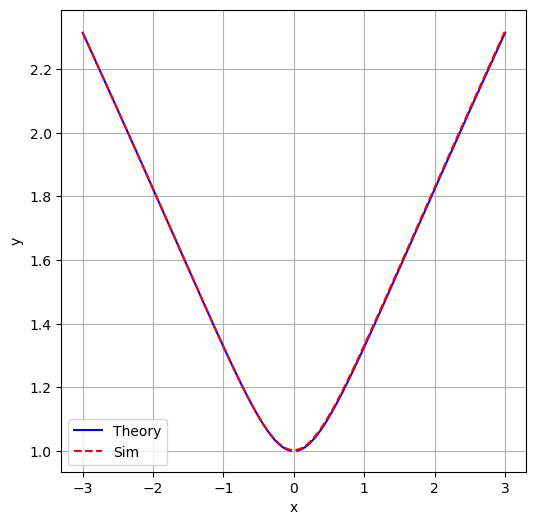
\includegraphics[width=\columnwidth]{plots/plot.png}
    \caption{Plot of the differential equation when $h=0.01$}
    \label{fig:Plot1}
    \end{figure}

\end{document}
